\chapter{Arquitectura de la solución}

En este capítulo vamos a describir la arquitectura que hemos diseñado para distribuir el bucle MAPE-K. Partimos de un sistema con una \textcolor{red}{división funcional ya definida}, por lo que será sencillo delimitar los componentes. El foco de este capítulo serán entonces los \textbf{conectores de \emph{software}}. Necesitamos establecer qué estrategias de comunicación utilizaremos para comunicar los componentes.

Comenzaremos dando una breve introducción a las arquitecturas de \emph{software} y los elementos que las componen. Después, describiremos la arquitectura de nuestra solución y el proceso que hemos seguido para llegar hasta ella.

\section{Arquitecturas de \emph{software}}

Según \cite{taylorSoftwareArchitectureFoundations2009}, la \textbf{arquitectura de un sistema \emph{software}} es el conjunto de todas las \textbf{decisiones principales de diseño} que se toman durante su ciclo de vida; aquellas que sientan las bases del sistema. Estas afectan a todos sus apartados: la funcionalidad que debe ofrecer, la tecnología para su implementación, cómo se desplegará, etc. En conjunto, definen una pauta que guía (y a la vez refleja) el diseño, la implementación, la operación y la evolución del sistema.

Todos los sistemas \emph{software} cuentan con una. La diferencia radica en si esta ha sido diseñada y descrita explícitamente o ha quedado implícita en su implementación. \cite{taylorSoftwareArchitectureFoundations2009} En el segundo caso es probable que, con el paso del tiempo, se ``erosione`` su arquitectura: se implementan funcionalidades sin respetar la estructura. También se olvida el por qué de ciertas decisiones. En general, se vuelve más difícil de mantener. Se convierte en una ''gran bola de barro''. \cite{footeBigBallMud1997}

Por tanto, es vital dedicar tiempo para definirla atendiendo a las necesidades de nuestro sistema. Una buena arquitectura es capaz dotar de estructura a nuestro sistema. \cite{martinCleanArchitectureCraftsman2018} Mientras se respete la arquitectura, y se mantenga actualizada, esta estructura. Una buena arquitectura nos ofrece una serie de ventajas, como facilitar su desarrollo, mayor extensibilidad.

\subsection{Componentes de una arquitectura}

Otra posible definición de arquitectura la encontramos en el estándar IEEE 42010-2011 \cite{ieeeStandard420102011Systems2011}: es "\emph{un conjunto de conceptos o propiedades fundamentales, personificados por sus elementos, sus relaciones, y los principios que guían su diseño y evolución}".

Podemos describirlas entonces usando tres conceptos: \cite{perryFoundationsStudySoftware1992}

    \begin{itemize}
        \item \textbf{Componentes} (o elementos): Son las piezas fundamentales que conforman el sistema. Representan las unidades de funcionalidad de la aplicación. Se utilizan para describir \textbf{\emph{qué}} partes componen el sistema. Por ejemplo: un módulo, un servicio web...

        \item \textbf{Forma}: El conjunto de propiedades y relaciones de un elemenento con otros o con el entorno de operación. Describe \textbf{\emph{cómo}} está organizado el sistema. Por ejemplo: un servicio A contacta con otro, B, usando una llamada HTTP.

        \item \textbf{Justificación}: Razonamiento o motivación de las decisiones que se han tomado. Responden al \textbf{\emph{por qué}} algo se hace de una manera determinada. Normalmente no pueden deducirse a partir de los elementos y la forma, por lo que es necesario describirlos explícitamente.

    \end{itemize}

\subsubsection{Elementos}

El primer tipo de elemento que debemos tratar son los componentes. Según \cite{taylorSoftwareArchitectureFoundations2009}, los \textbf{componentes} son ``elementos arquitectónicos que encapsulan un subconjunto de la funcionalidad y/o de los datos del sistema``.
Dependiendo de las características de nuestro sistema (y del nivel de abstracción que usemos) pueden tomar distintas formas: objetos, módulos dentro un mismo proceso, servicios distribuidos, etc.

\begin{wrapfigure}{r}{0.40\linewidth}
  \centering
  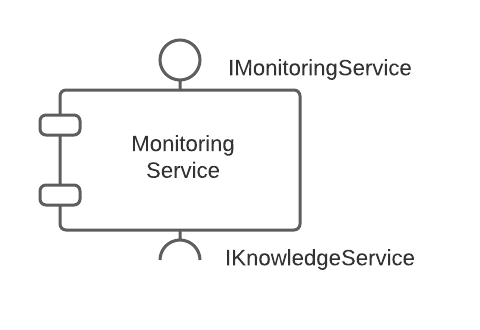
\includegraphics[scale=0.8]{cap_arquitectura/images/componente-ejemplo}
  \caption{El servicio de monitorización representado como un componente. Ofrece una interfaz (\emph{IMonitoringService}) y depende de otra para funcionar (\emph{IKnowledgeService}).}
  \label{fig:componenteEjemplo}
\end{wrapfigure}

Los componentes exponen una \textbf{interfaz} que permite acceder a la funcionalidad o datos que encapsulan. A su vez, también declaran una serie de \textbf{dependencias} con interfaces de otros. Allí se incluyen todos los elementos que requieren para poder funcionar. En la figura \ref{fig:componenteEjemplo} tenemos un ejemplo. \emph{Monitoring Service} expone la interfaz \emph{IMonitoringService}. Para poder funcionar, depende de un componente que ofrezca \emph{IKnowledgeService}.

Por si solos, estos componentes independientes no aportan mucho valor. Más bien son la unidad básica de composición: podemos combinar varios de ellos para que trabajen conjuntamente y realicen tareas más complejas. Así, podemos \textbf{componer sistemas}. \cite{mehtaTaxonomySoftwareConnectors2000} La integración y la interacción entre ellos son aspectos clave que debemos abordar.

Para que dos o más componentes puedan interactuar, necesitamos definir un mecanismo de comunicación. Recurrimos entonces a los \textbf{conectores}. Se trata de elementos arquitectónicos que nos ayudan a definir y razonar sobre la comunicación entre componentes. En la figura \ref{fig:componentesYConectorEjemplo} mostramos una representación de la necesidad de comunicación entre dos componentes a través de un conector. No se ha especificado todavía ningún detalle sobre cómo se implementará. Así, podemos estudiar la arquitectura y elegir los mecanismos adecuados para cada interacción del sistema. \cite{taylorSoftwareArchitectureFoundations2009}.

%% TODO: Los conectores son application-independent. No dependen de la funcionalidad de la aplicación.
%% TODO: Hablar de la cardinalidad de los conectores.

\begin{figure}[h!]
  \centering
  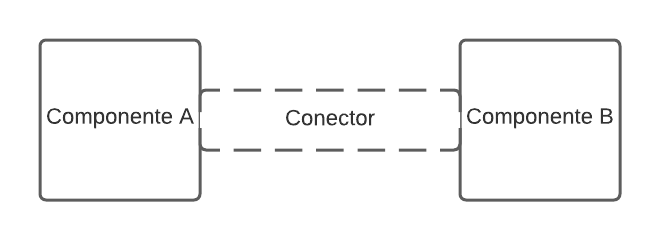
\includegraphics[scale=0.78]{cap_arquitectura/images/conector}
  \caption{Ejemplo de comunicación de dos componentes a través de un conector.}
  \label{fig:componentesYConectorEjemplo}
\end{figure}

Internamente, los conectores están compuestos por uno o más \textbf{conductos} o canales. A través de estos se lleva a cabo la comunicación entre los componentes. Hay una gran variedad de conductos posibles: comunicación interproceso, a través de la red, etc. Clasificamos los conectores según la complejidad de los canales que utilizan \cite{mehtaTaxonomySoftwareConnectors2000}:

\pagebreak

\begin{itemize}
    \item \textbf{Conectores simples}: solo cuentan con un conducto, sin lógica asociada. Son conectores sencillos. Suelen estar ya implementados en los lenguajes de programación. Por ejemplo: una llamada a función en un programa o el sistema de entrada / salida de ficheros.

    \item \textbf{Conectores complejos}: cuentan con uno o más conductos. Se definen por composición a partir de múltiples conectores simples. Además, pueden contar con funcionalidad para manejar el flujo de datos y/o control. Suelen utilizarse importando \emph{frameworks} o librerias. Por ejemplo: un balanceador de carga que redirige peticiones a los nodos.
\end{itemize}

Por tanto, cuando hayamos decidido que dos componentes necesitan comunicarse, es momento de evaluar qué mecanismo de comunicación es más adecuado. Basándonos en nuestros requisitos, la arquitectura ya definida, y los mecanismos de despliegue que queremos usar, elegimos el conector apropiado. Podemos orientarnos con taxonomías como la de \cite{mehtaTaxonomySoftwareConnectors2000}.

\subsubsection{Forma}

\textcolor{red}{TODO:  - ¿Borrar?  Innecesario}

\subsubsection{Justificación}

\textcolor{red}{TODO:  - ¿Borrar?  Innecesario}

Una vez definidos los componentes, los conectores y las relaciones entre ellos, tendremos una representación del sistema. Pero se trata de una imagen incompleta. No cuenta con ciertos detalles del contexto que nos ayudan a entenderlo mejor. Un ejemplo podría ser qué alternativas se consideraron y por qué se descartaron en favor de la elegida. Tampoco contamos con detalles minuciosos que puedan guiar mejor la implementación.

Es decir, requerimos de un concepto adicional para describirlos en nuestra arquitectura: se trata de la \textbf{justificación}. \cite{perryFoundationsStudySoftware1992} Nos aporta detalles más precisos sobre el sistema que no se pueden representar como elementos o forma.

\subsection{Estilos arquitectónicos}

\textcolor{red}{TODO:  - ¿Borrar?  Innecesario}

\textcolor{red}{Podemos agrupar decisiones principales.}
